% This document is a playground for testing new commands before inserting them
% into the .sty file

\documentclass{scrartcl}

\usepackage{lilyglyphs}


%%%%%%%%%%%%%%%%%%%%%%%%
% Numbers and Dynamics %
%%%%%%%%%%%%%%%%%%%%%%%%

%\newcommand{\lilyNumber}[2][1.35]{\lilyText[#1]{#2}}

% general \time n/m command (prints time signature as a fraction in emmentaler font)
\newcommand*{\lilyTimeSignature}[2]{$\frac{\mbox{\lilyText{#1}}}{\mbox{\lilyText{#2}}}$}



\begin{document}

\section*{Dynamic Letters}
	\lilyText{sffpzm1+2}
{	\LARGE
	\lilyText[scale=1.4]{sffpzm1+2 - , .}
}	
	
	lilyText \lilyText{sf} and lilyDynamics \lilyDynamics{sf} with default scaling.
	
	Compare sf with and without small space between:\\
	\lilyDynamics{rfz}\\
	\lilyDynamics{r\hspace{0.035ex}fz}\\
	\lilyRF* more text\\
	\lilyRFZ.
	
\section*{Numbers}
Numbers with scaling 1 suit like this: \lilyText{0 1 2 3 4 5 6 7 8 9} in a line.\\
If you want them like uppercase letters you should try a scaling of \lilyText[scale=1.3]{0 + 1 4 7} 1.3 instead.

\section*{Time Signatures}
	This is a normal Time signature: \lilyTimeSignature{3}{4}.
	
	As the plus sign is also directly accessible you can even
<<<<<<< HEAD
	write \lilyTimeSignature{3\,+\,7}{8+4} easily :-)

	%\lilyNumber
	
\section*{PGF/tikz}

Absatz, zusammen mit einem Notenkopf: 
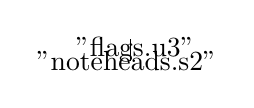
\begin{tikzpicture}
	\draw (0,0) node {\lilyGlyph{"noteheads.s2"}};
	\draw[semithick] (0.3ex,0) -- (0.3ex,0.8em);
	\draw (0.7ex,1ex) node {\lilyGlyph{"flags.u3"}};
\end{tikzpicture}

\Large
Neuer Absatz, zusammen mit einem Notenkopf: 
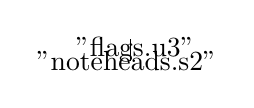
\begin{tikzpicture}
	\draw (0,0) node {\lilyGlyph{"noteheads.s2"}};
	\draw[semithick] (0.3ex,0) -- (0.3ex,0.8em);
	\draw (0.7ex,1ex) node {\lilyGlyph{"flags.u3"}};
\end{tikzpicture}

\normalsize
Neuer Absatz, zusammen mit einem Notenkopf: 
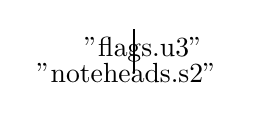
\begin{tikzpicture}[scale=2]
	\draw (0,0) node {\lilyGlyph{"noteheads.s2"}};
	\draw[semithick] (0.3ex,0) -- (0.3ex,0.8em);
	\draw (0.7ex,1ex) node {\lilyGlyph{"flags.u3"}};
\end{tikzpicture}

One sees: It is principally possible to combine graphical and textual elements with pgf/tikz,
but we definitely have to work on it some more: Especially it isn't scalable so far (explicitely or implicitely following text size)
=======
	write \lilyTimeSignature{3+7}{8+4} easily :-)
	
	One more option: \lilyTimeSignature{3}{8} \lilyText{+} \lilyTimeSignature{7}{4}. (note the space that the formula environment makes around it. Maybe this isn't the best approach?

	%Test the space after \lilyText
	This is a dynamics \lilyText[scale=1.4]{s} line. Space is added.\\
	Two letters in one command: \lilyText[scale=1.4]{sf}\\
	Space between dynamics and fullstop? \lilyText[scale=1.4]{s}.\\
	
	
>>>>>>> master
\end{document}